
\begin{figure*}[t]
\setlength{\tabcolsep}{.24\tabcolsep}
\begin{tabular}{|c|l|c||c|c|c|c|c||l|}
\hline
\multicolumn{3}{|c||}{Benchmarks} & \multicolumn{5}{|c||}{\ourtool} & Query by\\
\cline{1-8}
 ID & Source & \#Input Tables & Example Size & Rank & Time Cost (s) & Cost in Writing Examples (m) & \#Iterations & Output~\cite{Tran:2009}\\
 \hline
 \hline
 1 &Textbook Ex 5.1.1 & 4 &  & & & & & \\
 2 &Textbook Ex 5.1.2 & 4&  & & & & & \\
 3 &Textbook Ex 5.1.3 & 4&  & & & & & \\
 4 &Textbook Ex 5.1.4 & 4&  & & & & & \\
 5 &Textbook Ex 5.1.5 & 4&  & & & & & \\
 6 &Textbook Ex 5.1.6 & 4&  & & & & & \\
 7 &Textbook Ex 5.1.7 & 4&  & & & & & \\
 8 &Textbook Ex 5.1.8 & 4&  & & & & & \\
 9 &Textbook Ex 5.1.9 & 4&  & & & & & \\
 10 &Textbook Ex 5.1.10 & 4&  & & & & & \\
 11 &Textbook Ex 5.1.11 & 4&  & & & & & \\
 12 &Textbook Ex 5.1.12 & 4&  & & & & & \\
 13 &Textbook Ex 5.2.1 & 3 &  & & & & & \\
 14 &Textbook Ex 5.2.2 & 3&  & & & & & \\
 15 &Textbook Ex 5.2.3 & 3&  & & & & & \\
 16 &Textbook Ex 5.2.4 & 3&  & & & & & \\
 17 &Textbook Ex 5.2.5 & 3&  & & & & & \\
 18 &Textbook Ex 5.2.6 & 3&  & & & & & \\
 19 &Textbook Ex 5.2.7 & 3&  & & & & & \\
 20 &Textbook Ex 5.2.8 & 3&  & & & & & \\
 21 &Textbook Ex 5.2.9 & 3&  & & & & & \\
 22 &Textbook Ex 5.2.10 & 3&  & & & & & \\
 23 &Textbook Ex 5.2.11 & 3&  & & & & & \\
 24 &Forum Question 1 & &  & & & & & \\
 25 &Forum Question 2 & &  & & & & & \\
 26 &Forum Question 3 & &  & & & & & \\
 27 &Forum Question 4 & &  & & & & & \\
 28 &Forum Question 5 & &  & & & & & \\
\hline
\end{tabular}
\Caption{{\label{tab:results} Experimental results of SQL query synthesis.
Column ``Benchmarks'' describes the characteristics of our benchmarks. Sub-column ``\#Input Tables''
shows the number of input tables in each benchmark. Column ``\ourtool'' shows
\ourtool's results. Sub-column ``Example Size''
shows the number of tuples (i.e., rows) in all example input and output tables.
Sub-column ``Rank'' shows the absolute
rank of the correct SQL query in \ourtool's output.
``\textbf{X}'' means \ourtool fails to produce a correct answer.
Sub-column ``Cost in Writing
Examples (m)'' shows the total time cost of writing sufficient
examples in minutes. Sub-column ``\#Iterations'' shows the number of
interactive rounds in using \ourtool to obtain the correct query.
Column ``Query by Output'' shows the results of using an existing
technique, called
\textit{Query by Output} (QBO)~\cite{Tran:2009}. In this column,
``\textbf{Y}''  means QBO produces the correct SQL query, and ``\textbf{N}''
means QBO fails to produce the correct query.
Since QBO was implemented as a special case in \ourtool; its
time cost is similar to \ourtool and is omitted for brevity.
}}
\end{figure*}


\section{Evaluation}
\label{sec:evaluation}
\vspace{-1mm}

%\enlargethispage{5pt}

We evaluated four aspects of \ourtool's effectiveness,
answering the following research questions:

\begin{itemize}
\item What is the success ratio of \ourtool in synthesizing
SQL queries? (Section~\ref{sec:ratio}).
%Is the supported SQL subset expressive enough to describe a variety of queries?
\item How long does it take for \ourtool to
synthesize a SQL query? (Section~\ref{sec:performance}).
\item How much human effort is needed to write sufficient
input-output examples for SQL synthesis? (Section~\ref{sec:human}).
\item How does \ourtool's effectiveness compare to
existing SQL query inference techniques? (Section~\ref{sec:comparison}).
\end{itemize}





\vspace{-1mm}
\subsection{Benchmarks}
\vspace{-1mm}

%We collected benchmarks from two sources, and show them 
%in Figure~\ref{tab:results}.

Our benchmarks are shown in Figure~\ref{tab:results}.


\begin{itemize}
\item We used \allex SQL query related exercises
from a classic database textbook~\cite{cowbook}.
These exercises are from Chapter 5, which systematically
introduces the SQL language. We chose textbook exercises
because they are designed to
cover a wide range of SQL features. Some exercises
are even designed on purpose to be challenging and to cover some less realistic,
corner cases in using SQL. 
%all exercises are about
%writing a SQL query that retrieve data from a database.
We used \allex exercises that can be answered using standard
SQL language features without any vendor-specific
features or user-defined numeric functions.
As shown in Figure~\ref{tab:results},
many textbook exercises involve at least 3 tables. It was unintuitive
for us to write the correct query by simply looking at the problem
description.

\item We searched SQL query related questions raised by real-world
database users from 3 popular online forums~\cite{stackoverflow,
tutorialized, dbjournal}.
We focused on questions about how to write queries
using standard SQL features.
We excluded questions that were vaguely described or were obviously
wrong, and discarded questions that had been proved
to be unsolvable by using SQL (e.g., computing a
transitive closure).
We collected \pnum non-trivial forum questions
(all questions are available at:~\cite{forumq}), among which
two questions even did not receive any reply on the forum.
Writing a good forum post is often harder than seeking 
information from internet or asking
a SQL expert (since the post has to clearly 
describe the problem), and these end-users had already tried but
failed to find the correct SQL query before they wrote the post.
\end{itemize}



\vspace{-2mm}
\subsection{Evaluation Procedure}
\vspace{-1mm}

We used \ourtool to solve each textbook exercise and forum
question. If an exercise or problem
was associated with example input and output,
we directly applied \ourtool on those examples.
Otherwise, we manually wrote some examples.
All examples are written by the second author
of this paper, who is not \ourtool's major developer.
%of a graduate
%student (whose research field is not database-related) at the
%University of Washington rather than
%\ourtool's developers.

In the evaluation, the \ourtool user wrote examples in
plain text files using CSV format. \ourtool parses the
files, and automatically infers the data type
of each column based on the provided values.

We checked \ourtool's correctness by comparing its
output with the expected SQL queries.
For textbook exercises, we compared \ourtool's output with
their correct answers. For forum questions, we first
checked \ourtool's output with the confirmed answer
in the same post, if there is any. Otherwise, we
manually wrote the correct SQL query and
compared it with \ourtool's output.
%determined
%whether \ourtool can produce it.
%the output query can fulfill
%the query task or not.

For some textbook exercises and forum questions,
if \ourtool inferred a SQL query that satisfied the input-output
examples but did not behave as expected,
we manually found an input on which the
SQL query mis-behaved and re-applied \ourtool to the new input. We
repeated this process and recorded the total number of
interactions.
% before \ourtool output a correct SQL query.


Our experiments were run on a 2.5GHz Intel Core i5 Mac Mini
with 4GB physical memory, running OS X Version 10.8.3.





\vspace{-2mm}
\subsection{Results}
\vspace{-1mm}

Figure~\ref{tab:results} summarizes our experimental results.

\subsubsection{Success Ratio}
\label{sec:ratio}


\ourtool synthesized correct SQL queries for \solexnum  out of
the \exnum textbook exercises and 
all \pnum forum questions.
We did not come across any benchmark
that can be expressed in our SQL subset,
but our algorithm failed to infer the correct query.
%The 20 successful benchmarks covered each
%supported SQL feature (Figure~\ref{fig:syntax}) at least once.
\ourtool failed to solve 8 textbook exercises,
because these exercises required to write
complex existential sub-queries in the join conditions
using the \CodeIn{IN} and \CodeIn{NOT EXIST} keywords,
which are not currently supported by \ourtool.
Compared to the textbook exercises, the \pnum
forum questions come from more realistic use cases,
and can be expressed in our SQL subset
and answered by \ourtool.
%; even 
%two questions did not received any reply on the forum
%but \ourtool still produced correct answers for them.



We also observed that our ranking strategy (Section~\ref{sec:ranking})
was surprisingly effective: for all benchmarks where
\ourtool produced a correct answer, it always ranked the correct
SQL query as the first suggestion.

%

\begin{figure*}[t]
  \centering
  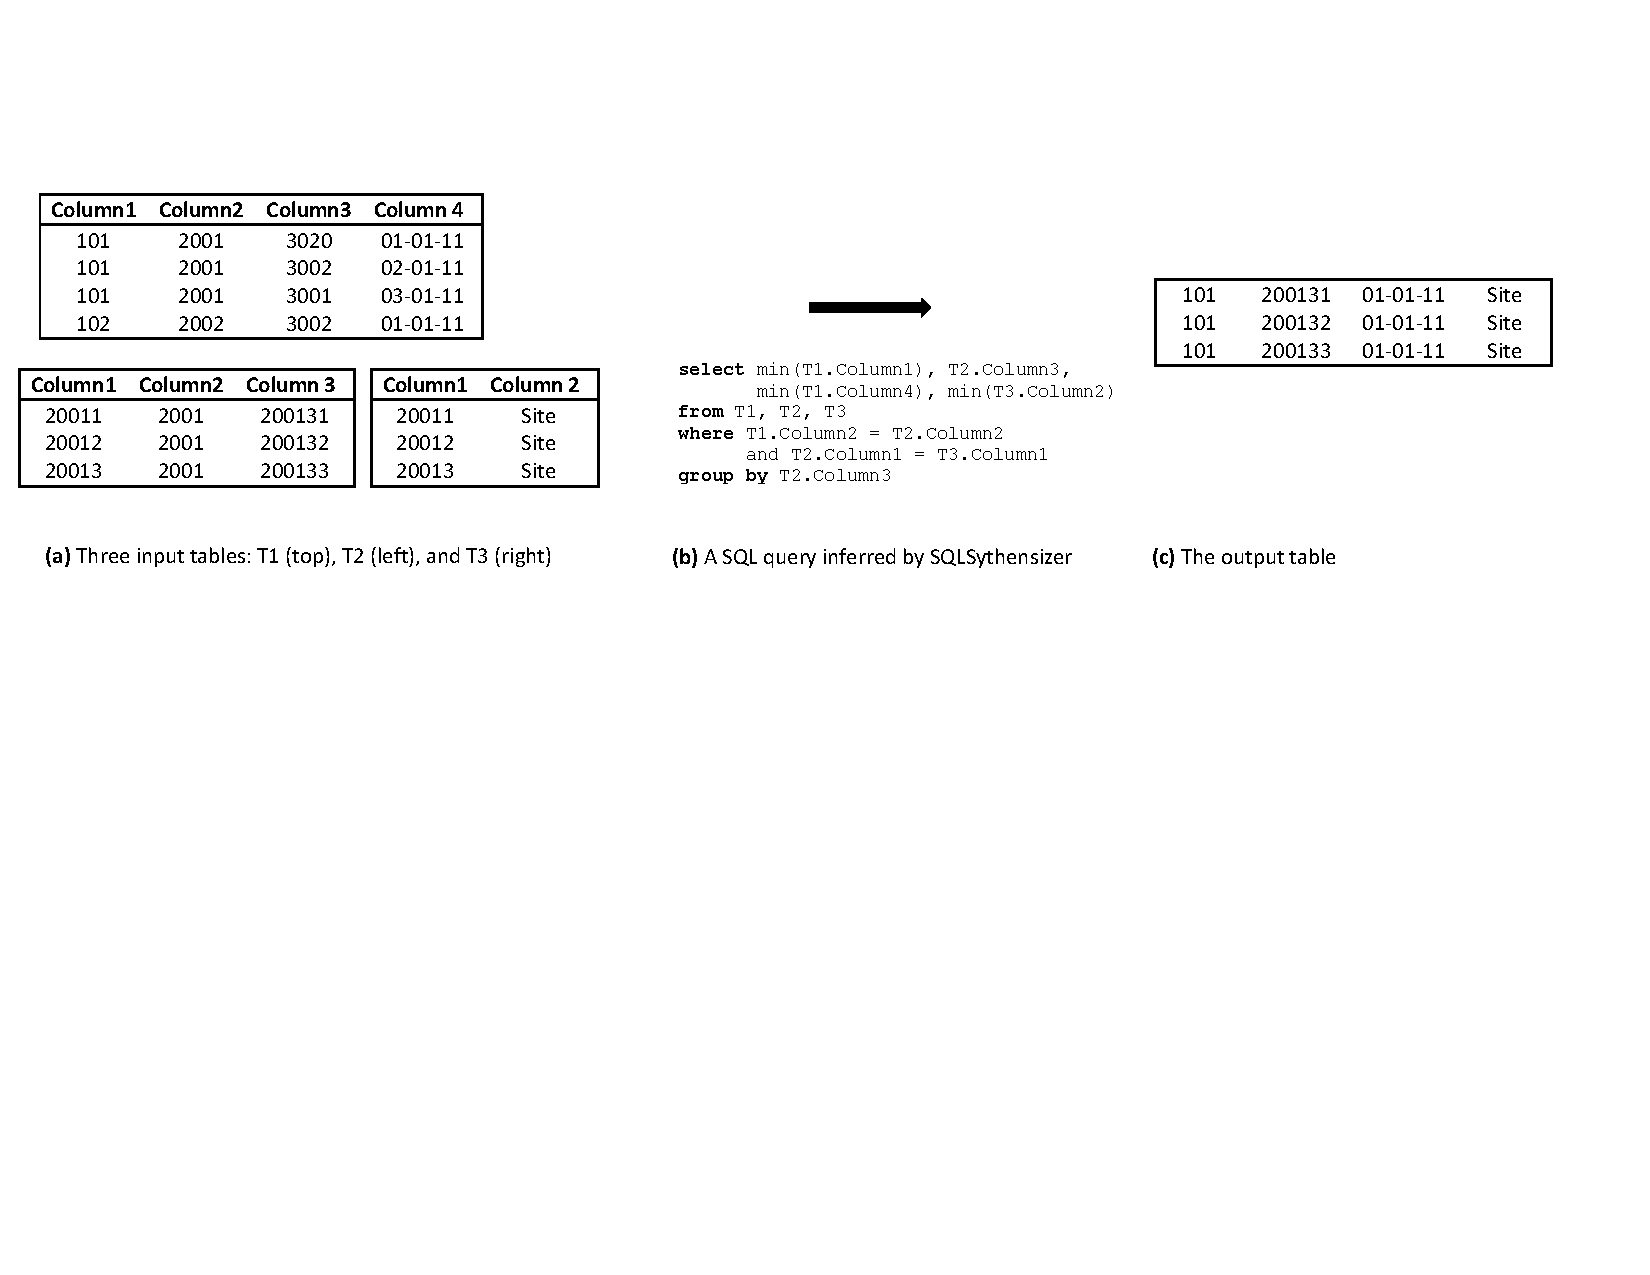
\includegraphics[scale=0.70]{example2}
  \vspace*{-1.0ex}\caption {{\label{fig:example2} Input-output
  examples ((a) and (c)) taken from an online SQL help forum
  thread. \ourtool automatically sythensizes 6 SQL queries that
  can produce the output table from the three input tables.
  (b) shows the highest ranked SQL query.
}}
\end{figure*}

We use a real SQL question from
an online forum\footnote{\url{http://forums.tutorialized.com/sql-basics-113/join-problem-147856.html}} to illustrate
\ourtool's effectiveness.
The question was started by a novice user, who needed help to write a
SQL query to get result from three input tables. In this question, the
novice user described his required query in a few paragraphs of
English, but also include several small, representative input-output
examples as shown in Figure~\ref{fig:example2}, to better express
his intention. 
This question receives no replies as of April 2013 and we speculated that
writing a SQL query to join three tables to produce certain output results
is non-trivial.

We ran \ourtool on the input-output examples
in Figure~\ref{fig:example2}. The tool produced 6 valid answers
in less than 1 minutes, all of which satisfy the given examples. The
highest ranked SQL query is shown in Figure~\ref{fig:example2},
which is quite unintuitive to write. The SQL query in
Figure~\ref{fig:example2}
first joins three input tables
on columns \CodeIn{T1.Column2}, \CodeIn{T2.Column2},
\CodeIn{T2.Column1}, and \CodeIn{T3.Column1} using some
selected columns, and then aggregates the results based on
column \CodeIn{Table2.Column3}'s value. Finally, it
returns the minimal values of columns \CodeIn{T1.Column1}, \CodeIn{T1.Column4}, and \CodeIn{T3.Column2}
from each aggregated group as the results.




\subsubsection{Performance}
\label{sec:performance}

As shown in Figure~\ref{tab:results}, \ourtool
is very efficient.
On average,
including benchmarks that \ourtool failed to produce
a correct answer,
\ourtool took less than \avgtime seconds in total to
produce the results (min: 1, max: 120).
For 20 benchmarks on which \ourtool succeeded, the average
time cost was only \avgsucctime seconds (min: 1, max: 120). 
Among them, in the worst case, \ourtool took 120 seconds to synthesize a
correct SQL query for a complex forum question, which includes 4 tables
and 13 columns. \ourtool searched over 920 possible
queries and validated each of them on the examples before getting
the correct answer. Even so, \ourtool's speed is still acceptable
for most practical use-case scenarios.

%Most of the time cost is spent querying the backend
%database to validate the correctness of each synthesized SQL query.

%\ourtool's speed makes it an attractive tool to replace
%the role of the SQL experts, which
%enables end-users to solve their problems in a few
%minutes.

%\todo{caching might be helpful}



\subsubsection{Human Effort}
\label{sec:human}

We measured the human effort required to use \ourtool in two ways.
First, the time cost to write sufficient input-output examples. Second,
the number of interactive rounds in invoking \ourtool
to synthesize the correct SQL queries.

The human effort required in writing
input-output examples is reasonable. For
the 20 successful benchmarks, it took the user less than
\avgsucchum minutes on average to write sufficient examples
per benchmark (min: 1, max: 7). The
average example size is \avgsucctuple
(min: 8, max: 52).
To produce the correct SQL query,
\ourtool requires just \avgsuccround rounds of
interaction on average (min: 1, max: 5).
For 19 successful benchmarks, the number of interaction
rounds is 1 to 3. In general, the user
spent slightly more time on benchmarks involving
more tables or requiring more complex query conditions.
%The maximum number of examples
%required in any scenario over all possible interactions was 10.

We also observed that,
for 6 of the failed benchmarks, the user
gave up after spending 10 minutes adding
examples and
10 interaction rounds invoking \ourtool, since the synthesized
SQL queries in each round seemed to get closer to the expected
query but still differed in some parts.
For the remaining 2 failed benchmarks, the user immediately
concluded that \ourtool could not produce a correct
answer after 1 and 4 rounds, respectively;
because the synthesized SQL
query is significantly different than expected.
Such observation is driving us to improve \ourtool's
user experience. For example, as our future work,
we plan to enhance \ourtool to inform users
about the solvability of a problem
\textit{earlier}.

%systematically explore the complete space, as described in Section 5


\subsubsection{Comparison with an Existing Technique}
\label{sec:comparison}
We compared \ourtool with \textit{Query By Output} (QBO),
a technique to infer SQL
queries~\cite{Tran:2009} from query output.
We chose QBO because it is the most recent technique and also one
of the most accurate SQL query inference techniques in
the literature. QBO requires an example input-output pair, and
uses the decision tree algorithm~\cite{Quinlan:1986} to infer a query.
However, QBO has three limitations. First, 
it can only join two tables on their key columns (annotated by users), and requires
users to specify how to project the results
by annotating the projection columns.
Second, it uses the original tuple values
from the input tables as learning features, and can only
infer simple query conditions. Third, QBO does not support
many useful SQL features, such as aggregates, the \CodeIn{GROUP BY}
clause, and the \CodeIn{HAVING} clause.

We implemented QBO, annotated
each example table as it required, and ran it
on the same benchmarks. The results are shown in Figure~\ref{tab:results}.
QBO produced correct answers
for only 2 textbook exercises and none of the forum questions.
Benchmarks solved by QBO were also solved by \ourtool.
QBO's poor performance is primarily caused by its
limited support for learning join conditions,
query conditions, and many other SQL features.

We did not compare \ourtool with other techniques~\cite{Howe:2011,
abs-1208-2013, Harris:2011, Kandel:2011}, because
these techniques either require different input
(e.g., a query log~\cite{Khoussainova:2010, Howe:2011}
or a snippet of Java code~\cite{abs-1208-2013}), 
or produce completely different
output (e.g., an excel macro~\cite{Harris:2011}, or a
text editing script~\cite{Kandel:2011}) than \ourtool.
Thus, it is hard to conduct a meaningful comparison.

\vspace{-1mm}
\subsection{Experimental Discussion}
\vspace{-1mm}

\enlargethispage{5pt}

\noindent \textbf{\textit{Limitations.}}
The experiments indicate three major limitations
of \ourtool. First, some queries
cannot be formulated by our SQL subset
due to unsupported features. This limitation is expected.
Our future work
should address it by including more SQL
features in \ourtool. Second, \ourtool requires
users to provide noise-free input-output examples.
Even in the presence of a small amount of 
noises (e.g., a typo), \ourtool will declare failure.
%when it fails to infer a valid SQL query.
To overcome this limitation, we plan to improve \ourtool
's algorithm, making it more robust. Third,
\ourtool does not provide any guidance regarding
when the user should give up on \ourtool and assume
the SQL can not be synthesized by \ourtool.
%, and even suggest a fix
%to the noisy example.

\vspace{.5mm}
\noindent \textbf{\textit{Threats to Validity.}}
There are two major threats to validity
in our evaluation. First, the \exnum textbook exercises
and \pnum forum questions, though covering
a wide range of SQL features, may not be representative enough.
Thus, we cannot claim the results can be generalized to an
arbitrary use-case scenario. Second, our
experiments focused on evaluating \ourtool's generality 
and accuracy. A user study is needed to further investigate
\ourtool's usefulness.
%A user study is needed to eliminate this threat.
%To address this issue, we plan to conduct
%a user study in our future work.


\vspace{.5mm}
\noindent \textbf{\textit{Experimental Conclusions.}}
We have three chief findings: \textbf{(1)}
\ourtool is effective in synthesizing SQL queries
from relatively small examples.
\textbf{(2)} \ourtool is fast enough for practical use;
and it only needs a small amount of human
effort in writing examples;
\textbf{(3)} \ourtool produces significantly better results
than an existing technique~\cite{Tran:2009}.




